% 2012 年天津卷理科第 17 题：四棱锥 P-ABCD，PA⊥平面 ABCD。
% 来源 PDF：普通高考/2012/2012天津理.pdf，第 2 页（印面 776）第 1 栏。
% 图中 A 在底面前部居中，B 在其右后，C 在最右，D 在左后；虚线为被遮挡的棱 PA、PB、AD、AB、BC 与对角线 AC。
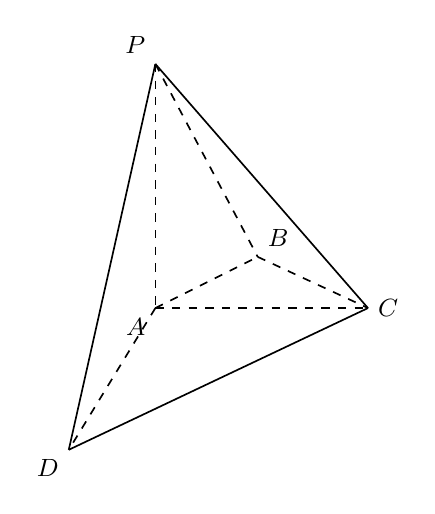
\begin{tikzpicture}[scale=1.0, semithick, font=\small]
  \coordinate (P) at (0.2,3.3);
  \coordinate (A) at (0.2,0.2);
  \coordinate (B) at (1.5,0.85);
  \coordinate (C) at (2.9,0.2);
  \coordinate (D) at (-0.9,-1.6);
  \draw (P) -- (C);
  \draw (P) -- (D);
  \draw (D) -- (C);
  \draw[dashed] (P) -- (A);
  \draw[dashed] (P) -- (B);
  \draw[dashed] (A) -- (B);
  \draw[dashed] (B) -- (C);
  \draw[dashed] (A) -- (C);
  \draw[dashed] (A) -- (D);
  \node[above left] at (P) {$P$};
  \node[below left] at (A) {$A$};
  \node[above right] at (B) {$B$};
  \node[right] at (C) {$C$};
  \node[below left] at (D) {$D$};
\end{tikzpicture}
